\documentclass{article}

\usepackage[utf8]{inputenc}
\usepackage[english]{babel}
\usepackage{amsthm} %lets us use \begin{proof}
\usepackage{amssymb} %gives us the character \varnothing
\usepackage{xcolor}
\usepackage{float}
\usepackage{braket}
\usepackage{multirow}
\usepackage{array}
\usepackage{mathtools}
\usepackage{geometry}
\usepackage{graphicx}
\geometry{margin=1in}

\title{Chapter 2: Quantum Dynamics in Hilbert Space} % Title of the assignment

\begin{document}

\maketitle

\section{Overview}

Chapter 2 introduces the reader to the Time-Dependent Schr{\"o}dinger equation (TDSE)
and defines the time propagator operator ($U(t,t_0)$). The two level system is
provided as an example of solving the TDSE and the corresponding time propagator operator
is determined. The interaction picture is used to simplify the
problem from the Schr{\"o}dinger picture and various properties are shown. Lastly,
the Greens function within the frequency domain is used to model the proposed
Wigner and Weisskopy of irreversible decay.

\section{Time-Evolution Operator with Time-Dependent Hamiltonian}{\label{sec:setup}}

Within the Schr{\"o}dinger picture, the TD wavefunction in the position space $\mathbf{x}$
is given by
\begin{equation}
  \psi(\mathbf{x},t) = \langle \mathbf{x}|\psi(t)\rangle
\end{equation}
and the TDSE will be defined as
\begin{equation}
  \frac{\partial|\psi(t)\rangle}{\partial t} = -\frac{i}{\hbar}H|\psi(t)\rangle
  \label{eqn:tdse}
\end{equation}
and solutions to Eqn \eqref{eqn:tdse} are the eigenvectors $|\phi_n(t)\rangle$ with corresponding
eigenvalues $E_n$. These eigenvections form a complete basis set and satisfy the completness
condition $\sum_n|\phi_n\rangle\langle\phi_n|=1$. We can expand the wavefunction
$\psi(t)$ within this basis,
\begin{equation}
  |\psi(t)\rangle = \sum_n|\phi_n\rangle\langle\phi_n|\psi(t)\rangle.
  \label{eqn:basis_expand}
\end{equation}

Substitution of Eqn \eqref{eqn:basis_expand} into the TDSE yields
\begin{equation}
  \frac{d}{dt}\langle \phi_n|\psi(t)\rangle = -\frac{i}{\hbar}E_n\langle\phi_n|\psi(t)\rangle,
  \label{eqn:tdse_basis}
\end{equation}
which is 1st-order differential equation with the solution
\begin{equation}
  \langle\phi_n|\psi(t)\rangle = \sum_ne^{-\frac{iE_n}{\hbar}(t-t_0)}|\phi_n\rangle
  \langle\phi_n|\psi(t_0)\rangle.
  \label{eqn:time_soln}
\end{equation}

The general time evolution operator is defined as
\begin{equation}
  |\psi(t)\rangle = U(t,t_0)|\psi(t_0)\rangle.
  \label{eqn:time_op}
\end{equation}

A few properties of the time evolution operator are that $U(t_0,t_0)=1$
and unitary $U^{\dagger}U=1$. The usefulness of this operator provides the means to solve the
time evolution of the system in general without needing specific initial conditions.
Hence, the TDSE only needs to be solved once with the corresponding $U(t,t_0)$ which
may operate on any intial state $|\psi(t_0)\rangle$. Based on Eqn \eqref{eqn:time_soln} and
\eqref{eqn:time_op}, the time evolution operator is
\begin{equation}
  U(t,t_0) = \sum_n|\phi_n\rangle e^{-\frac{iE_n}{\hbar}(t-t_0)}\langle\phi_n|.
  \label{eqn:time_evol}
\end{equation}

The current form of $U(t,t_0)$ is limited to the representation of the Hamiltnian $H$
and a general form is provided for greater flexibility. This will allow semiclassical
approximations. The general form can be obtained by the concept of a function of an
operator via Taylor series expansion. Given function $f(A)$ for operator $A$, the Taylor
series can be seen as
\begin{align}
  f(A) \equiv \sum^{\infty}_{p=0}\frac{f^{(p)}(0)}{p!}x^p \\
  f(A) = \sum^{\infty}_{p=0}\frac{f^{(p)}(0)}{p!}x^p \equiv f(a_j)|\alpha_j\rangle\langle\alpha_j
  \label{eqn:op_func}
\end{align}

With Eqns \eqref{eqn:time_evol} and \eqref{eqn:op_func}, the $U(t,t_0)$ is recasted into the form
\begin{equation}
  U(t,t_0) = e^{-\frac{i}{\hbar}H(t-t_0)}.
\end{equation}

\subsection{Two-level System Example}

Section \ref{sec:setup} reviews the TD quantum mechanic equations and introduces the
generalized time evolution operator. With the tools, an example of the time evolution
operator is demonstrated for a coupled two-level system ($|\phi_a\rangle$ and $|\phi_b\rangle$),
with energies $\epsilon_a$ and $\epsilon_b$, and a coupling $V_{ab}$, represented by the
Hamiltonian
\begin{equation}
  H =
  \begin{pmatrix}
    \epsilon_a & V_{ab} \\
    V_{ba} & \epsilon_b
  \end{pmatrix}
  \label{eqn:two_level_H}
\end{equation}
where $V_{ab} - V*_{ba} = |V_{ab}|E^{-i\chi},\; 0 <\chi < 2\pi$. This can be made into
an eigenvalue problem
\begin{equation}
  H\begin{pmatrix}
  |\phi_a\rangle \\
  |\phi_b\rangle
  \end{pmatrix}
  =
  \begin{pmatrix}
    \epsilon_a & V_{ab} \\
    V_{ba} & \epsilon_b
  \end{pmatrix}
  \begin{pmatrix}
  |\phi_a\rangle \\
  |\phi_b\rangle
  \end{pmatrix}
  =\epsilon_{\pm}
  \begin{pmatrix}
  |\phi_a\rangle \\
  |\phi_b\rangle
  \end{pmatrix}
\end{equation}

Diagonalize the Hamiltonian,
\begin{align}
  \text{det}(H-\lambda\mathbf{1}) &= 0 \\
  (\epsilon_a-\lambda)(\epsilon_b-\lambda) - |V_{ab}|^2 &= 0 \\
  \lambda^2 -\lambda(\epsilon_a+\epsilon_b) + \epsilon_a\epsilon_b
  - |V_{ab}|^2 &= 0 \\
  \lambda &= \frac{(\epsilon_a+\epsilon_b) \pm
    \sqrt{(\epsilon_a+\epsilon_b)^2 -4\epsilon_a\epsilon_b + 4|V_{ab}|^2}}{2}\\
  & = \frac{(\epsilon_a+\epsilon_b) \pm
    \sqrt{(\epsilon_a-\epsilon_b)^2 + 4|V_{ab}|^2}}{2} \nonumber \\
\end{align}
Eigenvectors corresponding to eigenvalues $\lambda$ are
\begin{equation}
  \begin{pmatrix}
    \frac{\epsilon_a-\epsilon_b\pm\sqrt{(\epsilon_a-\epsilon_b)^2+4|V_{ab}|^2}}{2V} & 1
  \end{pmatrix}
  \label{eqn:theta}
\end{equation}
The corresponding generalized eigenvectors ($|\psi_{\pm}\rangle$) are simply
linear compinations of $|\phi_a\rangle$ and $|\phi_b\rangle$
with the associated radiation phase $e^{\pm i\chi}$. These are rotated eigenvectors
from Eqn \eqref{eqn:theta}
\begin{equation}
  \begin{pmatrix}
    |\psi_+\rangle \\
    |\psi_-\rangle
  \end{pmatrix}
  =
  \begin{pmatrix}
    \cos(\theta) & \sin(\theta) \\
    -\sin(\theta)& \cos(\theta)
  \end{pmatrix}
  \begin{pmatrix}
    e^{-i\chi/2}|\phi_a\rangle \\
    e^{i\chi/2}|\phi_b\rangle
  \end{pmatrix}
  =\begin{pmatrix}
  \cos(\theta)e^{-i\chi}|\phi_a\rangle + \sin(\theta) e^{i\chi}|\phi_b\rangle \\
  \cos(\theta)e^{-i\chi}|\phi_a\rangle - \sin(\theta) e^{i\chi}|\phi_b\rangle
  \end{pmatrix}
  \label{eqn:sup_eig}
\end{equation}

$\theta$ is a transformation angle that can be determined with Eqns
\eqref{eqn:theta} and \eqref{eqn:sup_eig}. The work is shown in the mathematica
notebook
\begin{equation}
  \tan 2\theta \equiv \frac{2|V_{ab}|}{\epsilon_a-\epsilon_b},\; 0<\theta<\pi/2
  \label{eqn:angle_transform}
\end{equation}

Within this basis, the time evolution operator is given by
\begin{equation}
  U(t,t_0) = |\psi_+\rangle e^{-\frac{i\lambda_+}{\hbar}(t-t_0)}\langle\psi_+|
  + |\psi_-\rangle e^{-\frac{i\lambda_-}{\hbar}(t-t_0)}\langle\psi_-|
  \label{eqn:time_2_level}
\end{equation}

\subsection{Progating the two-level system}

Suppose the system is at initial time $t_0=0$ in the $|\phi_a\rangle$ state
and the probability that the system is in $|\phi_a\rangle$ at time $t$.
\begin{equation}
  P_{ab}(t)\equiv |\langle\phi_b|\psi(t)\rangle|^2 = |\langle\phi_b|U(t,t_0)|\phi_a\rangle|^2
  \label{eqn:prob_time}
\end{equation}

The states $|\phi_a\rangle$ and $|\phi_b\rangle$ are defined as unit
vectors and the substitution of Eqn \eqref{eqn:time_2_level} into Eqn \eqref{eqn:prob_time}
will yield the probability to be in state $|\phi_a\rangle$ at a given time $t$.
From mathematica, the $P_{ab}(t)$ is given as
\begin{align}
  P_{ab}(t)&= \sin^2(2\theta)\sin^2\Bigg(\frac{\lambda_- - \lambda_+}{2\hbar}t\Bigg)
  \label{eqn:trig_identity}\\
  &=\frac{4|V_{ab}|^2}{4|V_{ab}|^2+(\epsilon_a-\epsilon_b)^2}
  \sin^2\Bigg(\sqrt{4|V_{ab}|+(\epsilon_a-\epsilon_b)^2}\frac{t}{2\hbar}\Bigg)
  \label{eqn:prob_final}
\end{align}

The step from Eqn \eqref{eqn:trig_identity} to \eqref{eqn:prob_final}
is using Eqn \eqref{eqn:angle_transform}, the trignometry identity
$\sin^22\theta + \cos^22\theta = 1$, and substituting in the eigenvalues $\lambda$.
This is left for the reader to derive. Figure \ref{fig:prob} is the plot of
the probability for various coupling constants $V_{ab}$.
%\begin{align*}
%  (\tan 2\theta & =  \frac{2|V_{ab}|}{\epsilon_a-\epsilon_b})^2 \\
%  \tan^2(2\theta) & = \frac{4|V_{ab}|^2}{(\epsilon_a-\epsilon_b)^2} \\
%  \sin^2(2\theta) + \cos^2(2\theta) & = 1 \\
%  \tan^2(2\theta) & = \frac{1}{\cos^2(2\theta)} - 1 \\
%  & = \frac{4|V_{ab}|^2}{(\epsilon_a-\epsilon_b)^2} \\
%  \frac{1}{\cos^2(2\theta)} & = \frac{4|V_{ab}|^2 + (\epsilon_a-\epsilon_b)^2}{(\epsilon_a-\epsilon_b)^2} \\
%  \cos^2(2\theta) & = \frac{(\epsilon_a-\epsilon_b)^2}{4|V_{ab}|^2 + (\epsilon_a-\epsilon_b)^2} \\
%  & = 1 - \sin^2(2\theta) \\
%  \sin^2(2\theta) & = \frac{4|V_{ab}|}{4|V_{ab}|^2 + (\epsilon_a-\epsilon_b)^2}
%\end{align*}
\begin{figure}[hbpt]
  \centering
  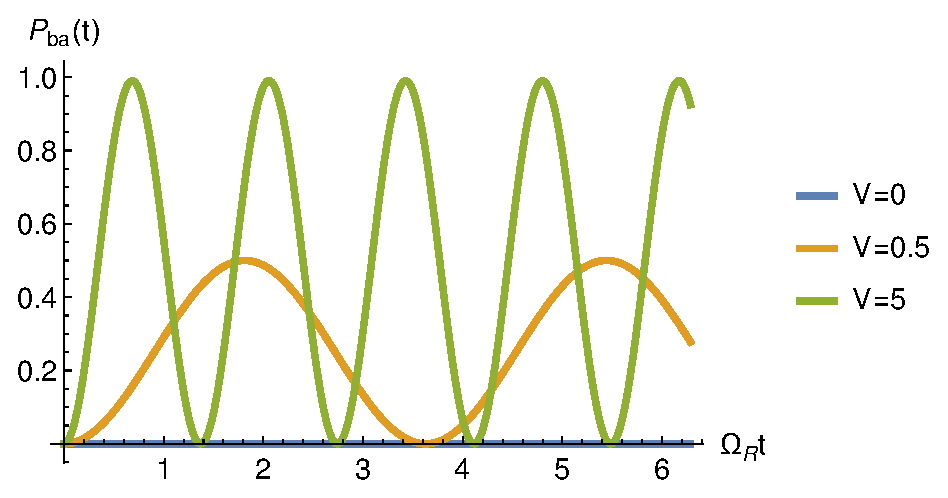
\includegraphics[scale=0.8]{prob2.eps}
  \caption{Rabi oscillation of the two level system for coupling constant $V_{ab}$ at 0, 0.5, and
  5.}
  \label{fig:prob}
\end{figure}
This is known as the Rabi formula and
\begin{equation}
  \Omega_{\text{R}}=\sqrt{4|V_{ab}|+(\epsilon_a-\epsilon_b)^2}/\hbar
\end{equation}
is the Rabi frequency.

\end{document}
